\subsection*
{\href{http://cst.mi.fu-berlin.de/intern/19606-P-MPP/Aufgaben/040202.html}
{Aufgabe 6: Stromverbrauch und Taktfrequenz}}

Folgende Tabelle zeigt die Abhängigkeit des Stromverbrauchs von der Taktfrequenz. Der DCOCLK-Taktgenerator wurde durch manuelle Modifikation der DCOCTL, BCSCTL1 und BCSCTL2 Register im Debug-Modus des Code Composers auf Frequenzen im Bereich von 100kHz bis 10MHz eingestellt. Anschließend wurde jeweils der Stromverbrauch des Controllers im RUN-Modus am in Reihe geschalteten Digitalmultimeter gemessen. Die Tabelle enthält alle Messwerte mit den entsprechenden Bit-Settings der Clock-Register.

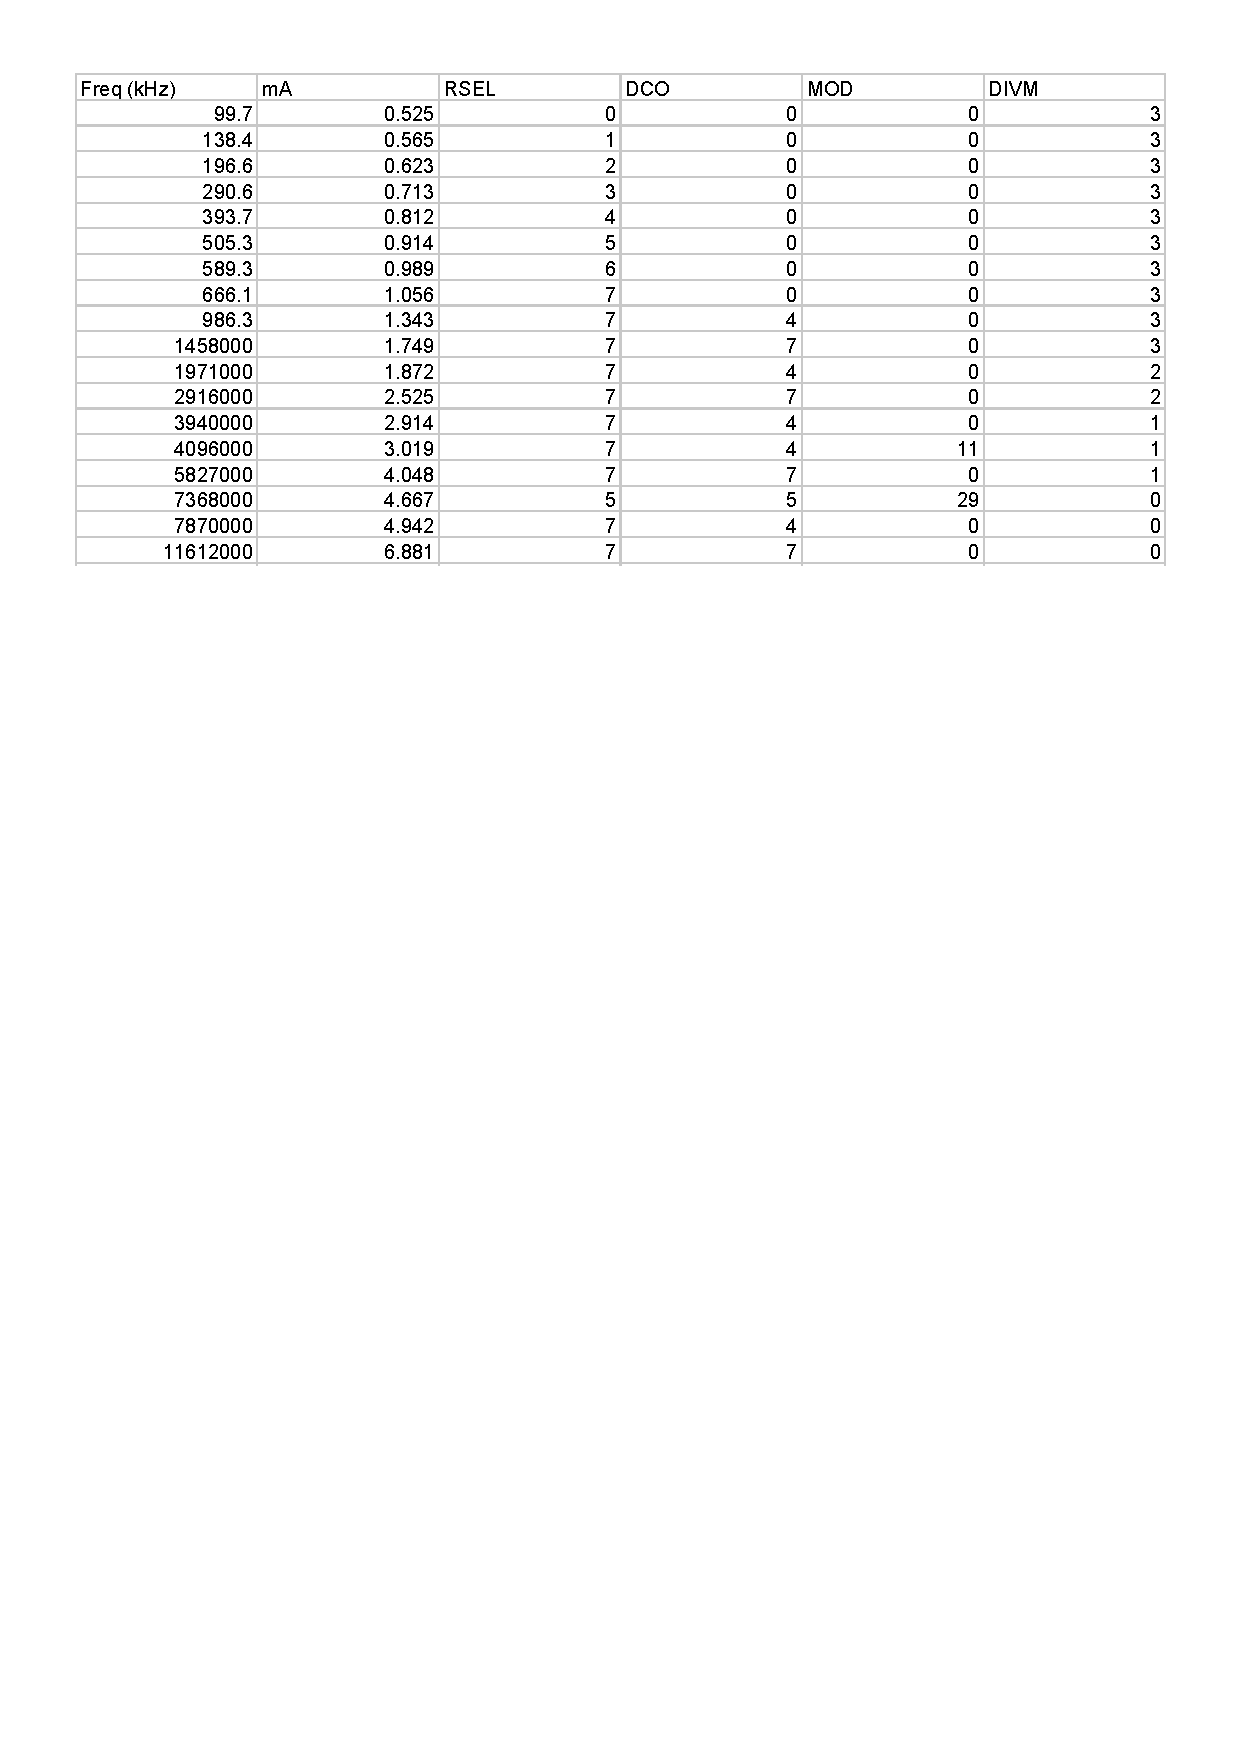
\includegraphics[width=\textwidth]{aufgaben/06/DCOCLK.pdf}
\\

Das Diagramm zeigt den Stromverbrauch (vertikal) im Verhältnis zur Taktfrequenz (horizontal) der MCLK an Hand obiger Messwerte. Der Stromverbrauch steigt nicht proportional sondern scheinbar exponentiell mit der Taktfrequenz.

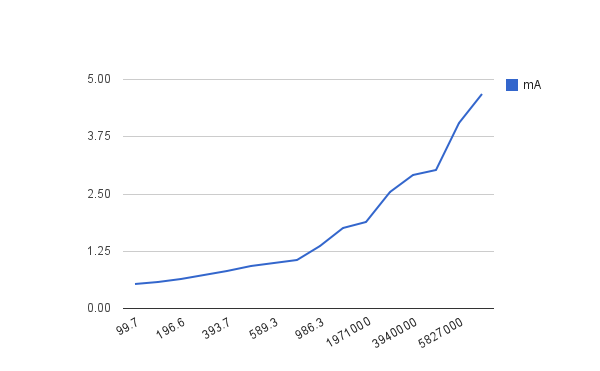
\includegraphics[width=0.93\textwidth]{aufgaben/06/chart_1.png}
